\documentclass{jsarticle}

\usepackage[dvipdfmx]{graphicx}
\usepackage{amsmath}

\title{
    学習済みtransformerモデルのコンテキスト拡張 \\
    における位置エンコーディング
}
\author{平田 蓮}
\date{2024年5月22日}

\begin{document}
\maketitle

\section{Attention機構}
    Attention機構は、入力トークンの特徴量を、
    他トークンとの「関係性」を加味しながら計算する仕組み。
    最終的なトークンの特徴量は、Attention機構を繰り返し通すことで形成される。
    各Attention機構では、前の段階で作られた特徴量からトークンごとに
    Query, Key, Valueの三種類のベクトルを構成する。

    それぞれのベクトルの意味のイメージは次の通り。
    \begin{description}
        \item[Query] 自身のトークンと関連性の強いトークンを参照する
        \item[Key] 各トークンのQueryに対して適切な自身のValueを返す
        \item[Value] トークンの「値」
    \end{description}

    まず、入力を得たAttention機構は、線形層を用いて各ベクトルを計算する。
    下図参照。
    \begin{figure}[h]
        \centering
        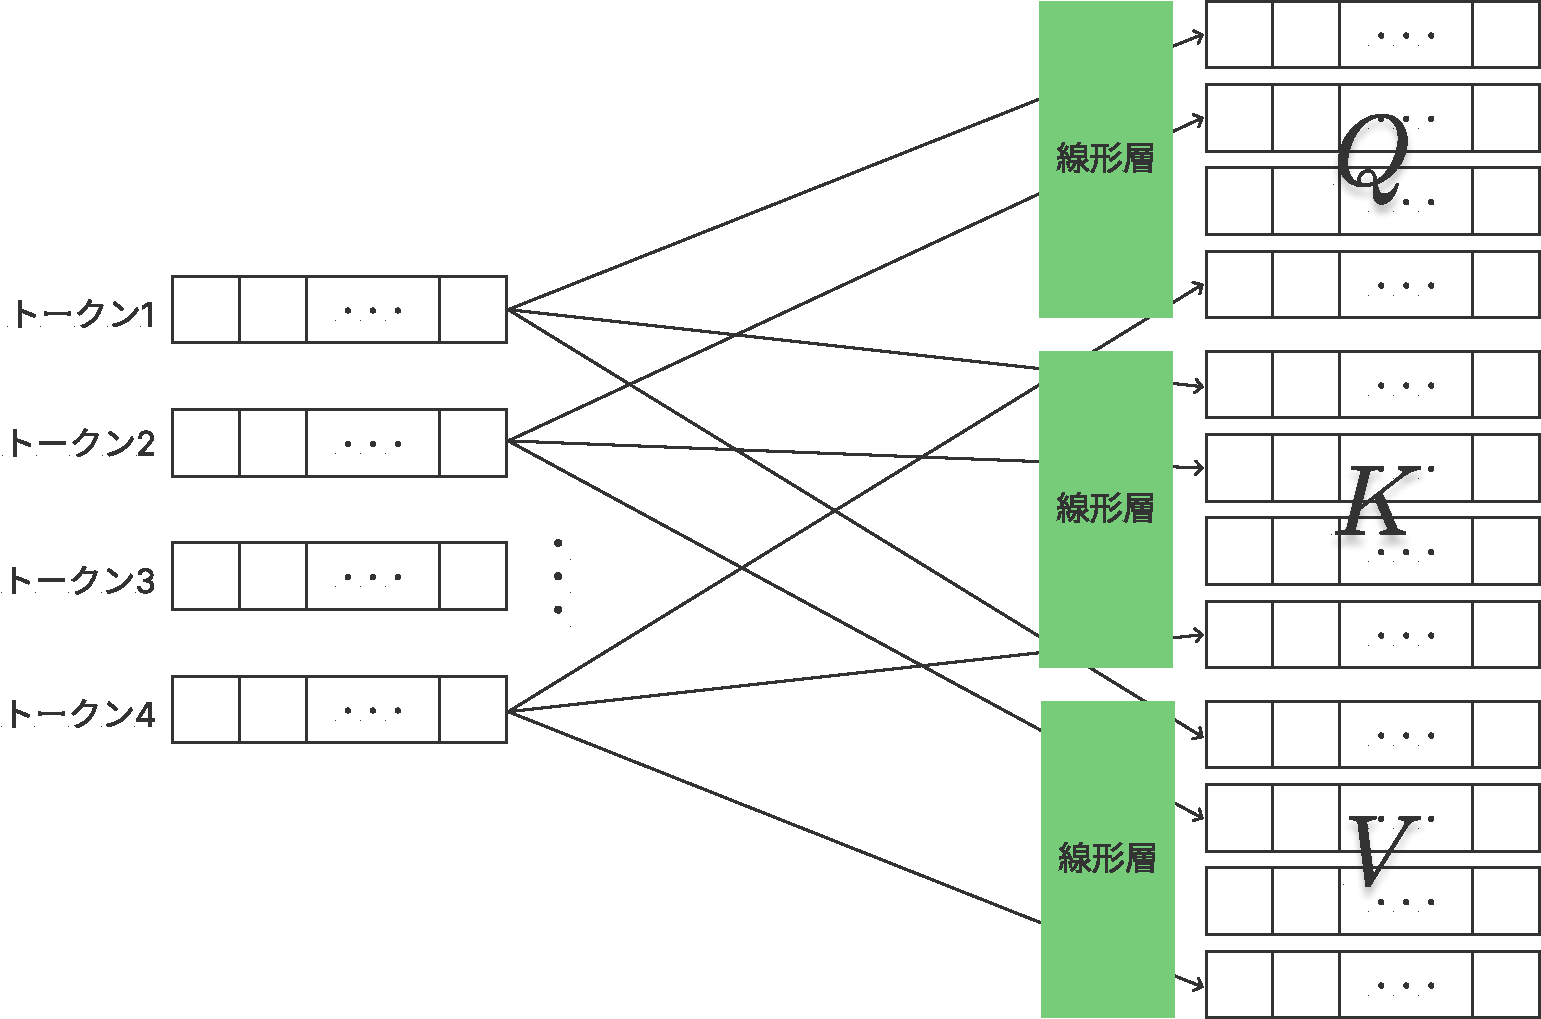
\includegraphics[width=.8\linewidth]{qkv.pdf}
        \caption{Query, Key, Valueの計算}
    \end{figure}

    次に、次の式に基づいてAttention行列$A$を計算する。
    \begin{align*}
        A = \mathrm{Softmax}\left(\frac{Q^t\!K}{\sqrt{d}}\right)
    \end{align*}
    $Q, K$はそれぞれ各トークンのQueryとKeyを並べた行列で、
    大きさはトークン数を$n$,
    埋め込みの次元を$d$とすると、
    $n\times d$である。
    $Q$と$K$を掛けることで各トークン同士の関係の強さを計算し、
    それを正規化したものが$A$である。
    $A$を計算した後、
    $AV$の各行が各トークンの特徴量として次のAttention機構に渡される。
    \begin{figure}[h]
        \centering
        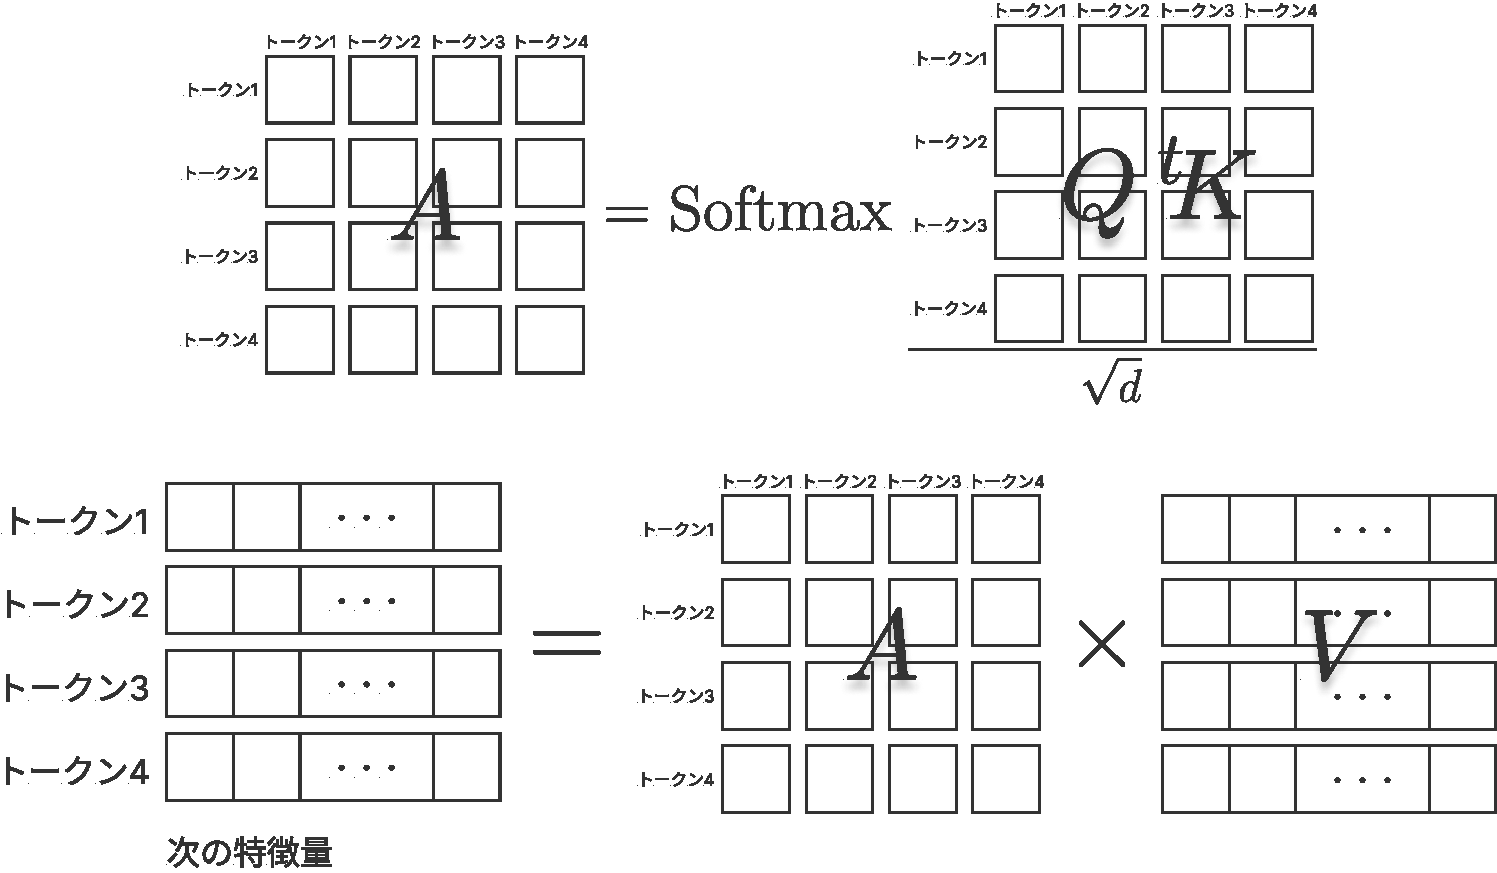
\includegraphics[width=.8\linewidth]{attention.pdf}
        \caption{Attention行列の計算}
    \end{figure}

\section{位置エンコーディング}
    Attention機構は、ベクトル同士の内積で特徴量が計算されるため、
    トークン同士の位置情報が失われる。
    よって、トークンの順番を入れ替えても同様の特徴量が得られてしまうという問題がある。
    これを解消するため、$A$を計算する際に位置情報を加味した計算を追加で行う。
    これを位置エンコーディングと呼ぶ。

    \subsection{絶対位置エンコーディング}
        Ashishら\cite{attention}が提案した位置エンコーディングを
        ここでは絶対位置エンコーディングと呼ぶ。
        絶対位置エンコーディングは、
        事前に計算されたベクトルを各トークンの特徴量に加算する。
        $i$番目のトークンの特徴量に対する位置エンコーディングの
        $j$番目の要素は次の式で計算される。
        \begin{align*}
            \mathrm{Positional Encoding} = \left\{
                \begin{aligned}
                    & \sin\left(\frac{i}{10000^{\frac{2j}{d}}}\right) \ (j\equiv 0 \mod 2) \\
                    & \cos\left(\frac{i}{10000^{\frac{2j}{d}}}\right) \ (j\equiv 1 \mod 2)
                \end{aligned}
                \right.
        \end{align*}

        絶対位置エンコーディングは、
        位置エンコーディングを加算することで元のベクトルの大きさが
        大きく変わらないように周期関数を採用しているが、
        周期が小さいと同じ位置エンコーディングが繰り返し出現してしまうため、
        周期を大きくしている。
        しかし、その場合$\sin$と$\cos$それぞれの勾配が小さい箇所では
        順番が入れ替わっても位置エンコーディングがほぼ変わらないという問題が発生する。
        これを回避するために、$\sin$と$\cos$を組み合わせている。

    \subsection{相対位置エンコーディング}
        絶対位置エンコーディングには次の改善点が挙げられる。
        \paragraph{時系列データは絶対位置よりも、他のトークンとの相対位置が重要}
            例えば日本語の文章で考えると、
            「私のペンが…」と「〇〇。私のペンが…」という二つのシーケンスでは
            「ペン」の位置が違うので絶対位置エンコーディングでは別の値となるが、
            実際は「私」「の」の次にあるという相対的な位置情報が大事である。
        \paragraph{学習データに無い長さの系列を処理できない}
            学習データに無い長さの系列をモデルに与えた時、
            後ろの方の絶対位置エンコーディングは学習が甘い状態であるため、
            適切な推論ができなくなることが確認されている。下図参照。
            \begin{figure}[h]
                \centering
                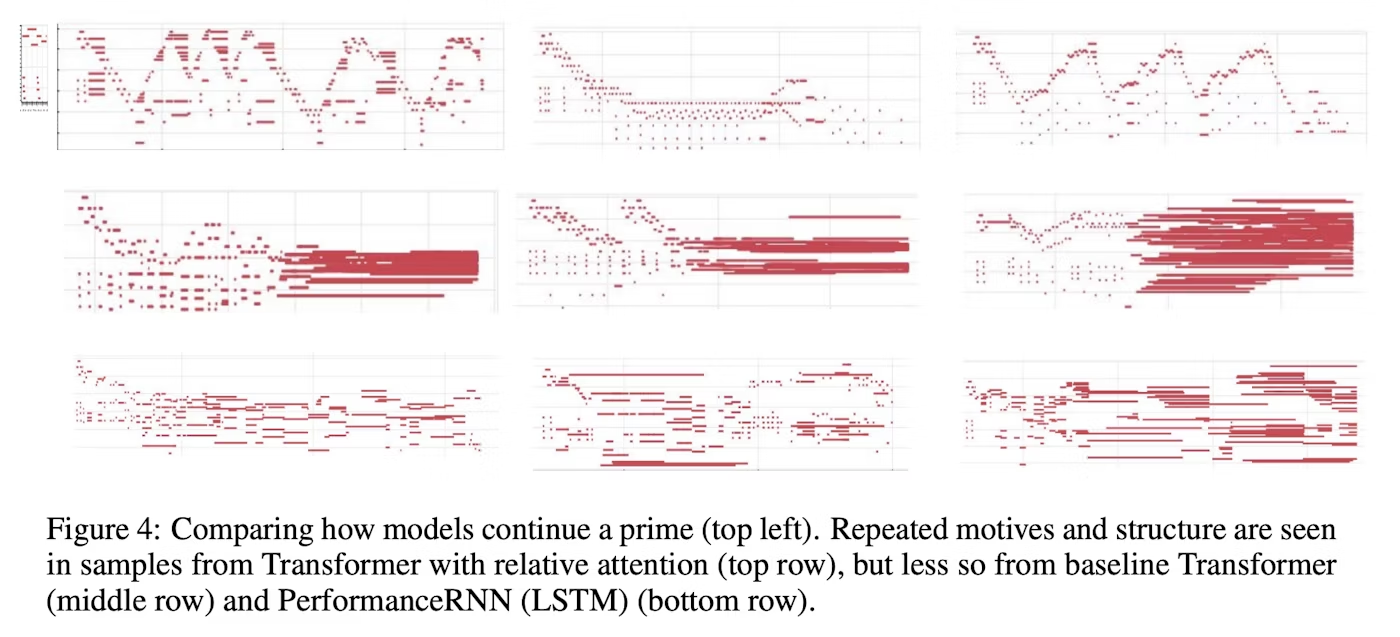
\includegraphics[width=.8\linewidth]{catastrophie.png}
                \caption{
                    Chengら\cite{catastrophie}は、
                    相対位置エンコーディングを用いたtransformerは
                    学習にない長さの系列の出力をうまくできないことを確認した。
                }
            \end{figure}

        これを踏まえ、Peterら\cite{relative}は相対位置エンコーディングを提案した。
        相対位置エンコーディングは下図に示すような行列であり、
        Attention行列を計算する際に$Q^t\!K$に加算される。
        相対位置エンコーディングの行列は、
        各Attention機構が固有に保持する距離ごとの埋め込みと、
        各トークンのQueryの内積で計算される。
        \begin{figure}[h]
            \centering
            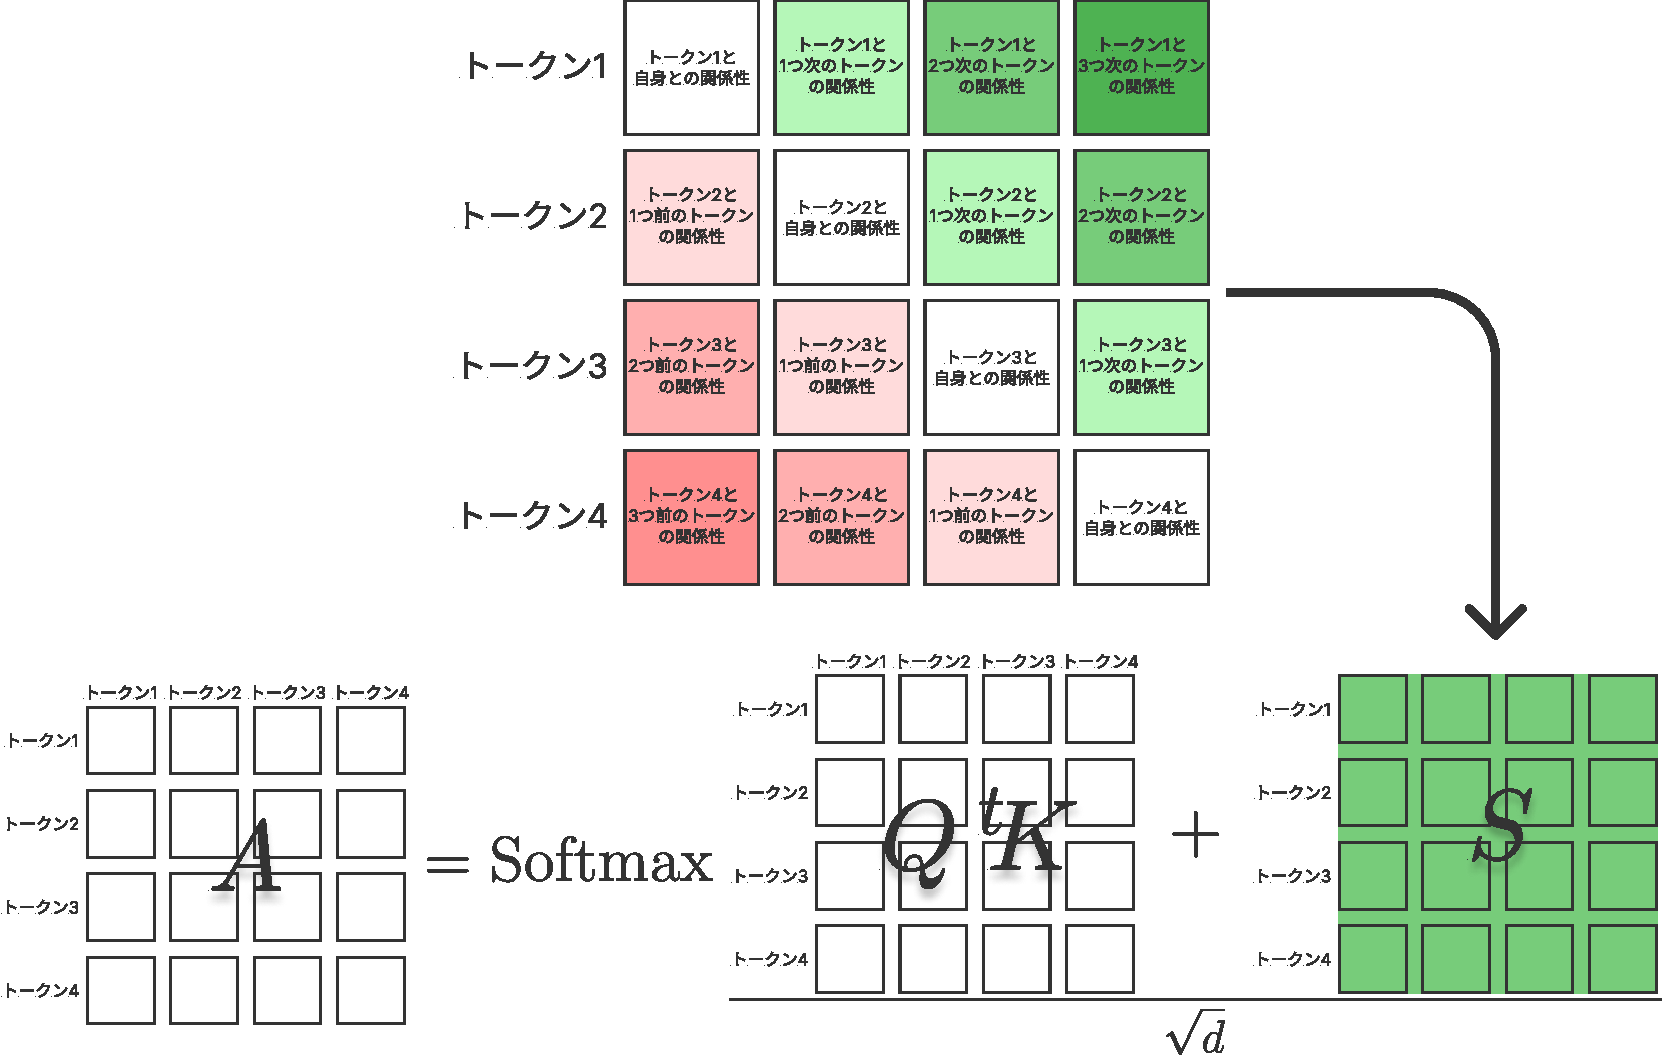
\includegraphics[width=.8\linewidth]{relative.pdf}
            \caption{相対位置エンコーディング}
        \end{figure}

    \subsection{RoPE}
        位置エンコーディングを加算ではなく乗算で行うアプローチ。
        LLaMAなどで用いられており、現在主流である。
        QueryとKeyに回転行列をかけて、ベクトルを回転させることで位置情報を乗せる。
        トークンの位置ごとに徐々に回転角を増していくため、
        相対位置情報も反映されていると考えられている。

        回転行列は、次の式で与えられる。
        \begin{align*}
            R &= \begin{pmatrix}
                    \cos m\theta_1 & -\sin m\theta_1 & 0 & 0 & \cdots & 0 & 0 \\
                    \sin m\theta_1 & \cos m\theta_1 & 0 & 0 & \cdots & 0 & 0 \\
                    0 & 0 & \cos m\theta_2 & -\sin m\theta_2 & \cdots & 0 & 0 \\
                    0 & 0 & \sin m\theta_2 & \cos m\theta_2 & \cdots & 0 & 0 \\
                    \vdots & \vdots & \vdots & \vdots & \ddots & \vdots & \vdots \\
                    0 & 0 & 0 & 0 & \cdots & \cos m\theta_\frac{d}{2} & -\sin m\theta_\frac{d}{2} \\
                    0 & 0 & 0 & 0 & \cdots & \sin m\theta_\frac{d}{2} & \cos m\theta_\frac{d}{2}
                \end{pmatrix} \\
            \theta_i &= 10000^{-\frac{2(i-1)}{d}} \ \left(i = 1, 2, \cdots, \frac{d}{2}\right)
        \end{align*}
        ここで、$m$はトークン位置である。
        つまり、トークン位置が後ろに行くほど、回転角が大きくなる。
        この回転行列はベクトルの$d$次元空間を2次元ずつ取って、
        その2軸が成す平面において回転させる。
        これを用いて計算した$Q' = R^t\!Q, K' = R^t\!K$により
        Attention行列を計算する。
        \begin{figure}[h]
            \centering
            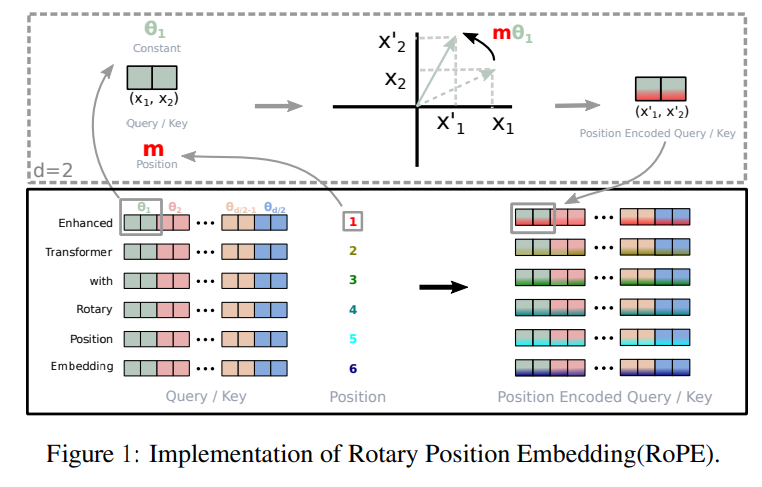
\includegraphics[width=.8\linewidth]{rope_image.png}
            \caption{RoPE\cite{rope}}
        \end{figure}

\section{コンテキスト拡張における位置エンコーディング}
    現在、学習済みのモデルのコンテキストを拡張する際の位置エンコーディングは、
    Scaled RoPEが主流に用いられている\cite{kaiokendev}。
    Scaled RoPEはその名の通り、
    RoPEをコンテキスト長の拡張に応じて引き伸ばす手法である。
    具体的には、上述の$m$を元のコンテキスト長$n$と
    新しいコンテキスト長$n'$を用いて$\displaystyle\frac{n}{n'}$倍する。

\section{展望}
    以下、研究の余地があると個人的に感じた内容を記す。

    \subsection{コンテキスト拡張における位置エンコーディングの別アプローチによる拡張}
        Scaled RoPEなどの既存の位置エンコーディングを引き伸ばす手法は、
        コンテキスト長を大きくした際に位置エンコーディングの「差」が小さくなってしまうため、
        極端にコンテキスト長を長くした際に位置エンコーディングの意味が薄れてしまう。
        これを回避したコンテキスト拡張の手法も提案されているが、
        既存の位置エンコーディングを拡張する手法は見つけれいないため、
        調査を継続したい。

    \subsection{位置エンコーディングのスパース性の調査}
        gpt-3の埋め込み次元は3072, 最大トークン長は8192である
        \footnote{https://platform.openai.com/docs/guides/embeddings/what-are-embeddings}。
        このときの絶対位置エンコーディングとRoPEの具体的な値を見てみる。
        \begin{figure}[h]
            \centering
            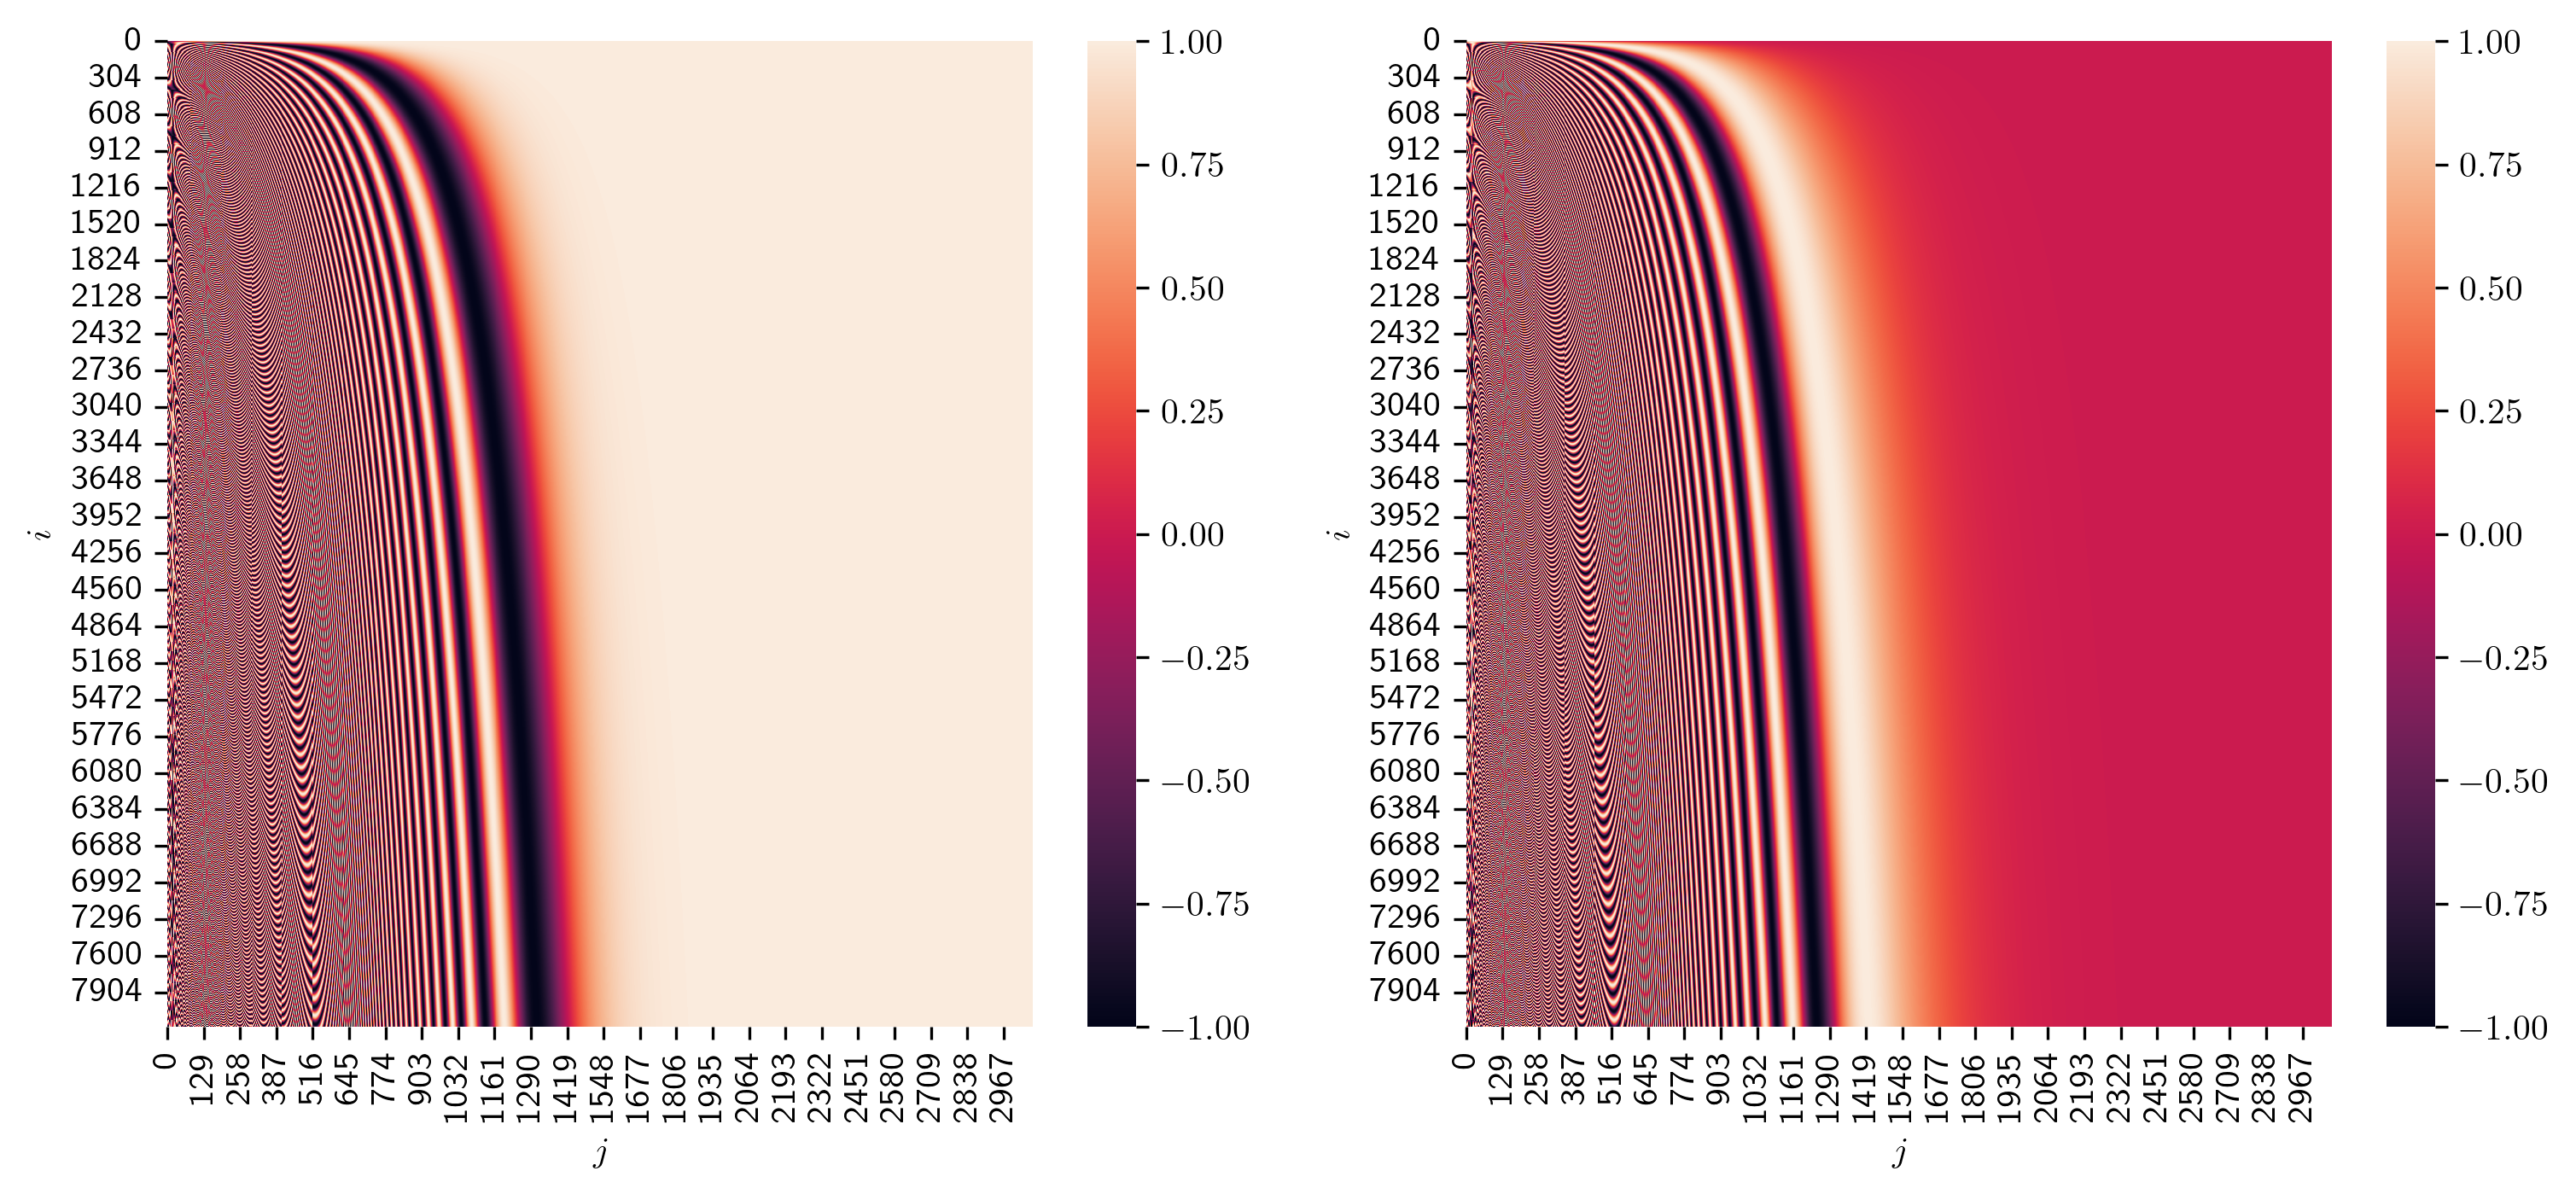
\includegraphics[width=1\linewidth]{absolute.png}
            \caption{
                絶対位置エンコーディングの値。
                $\cos$(左)と$\sin$(右)。
            }
        \end{figure}
        \begin{figure}[h]
            \centering
            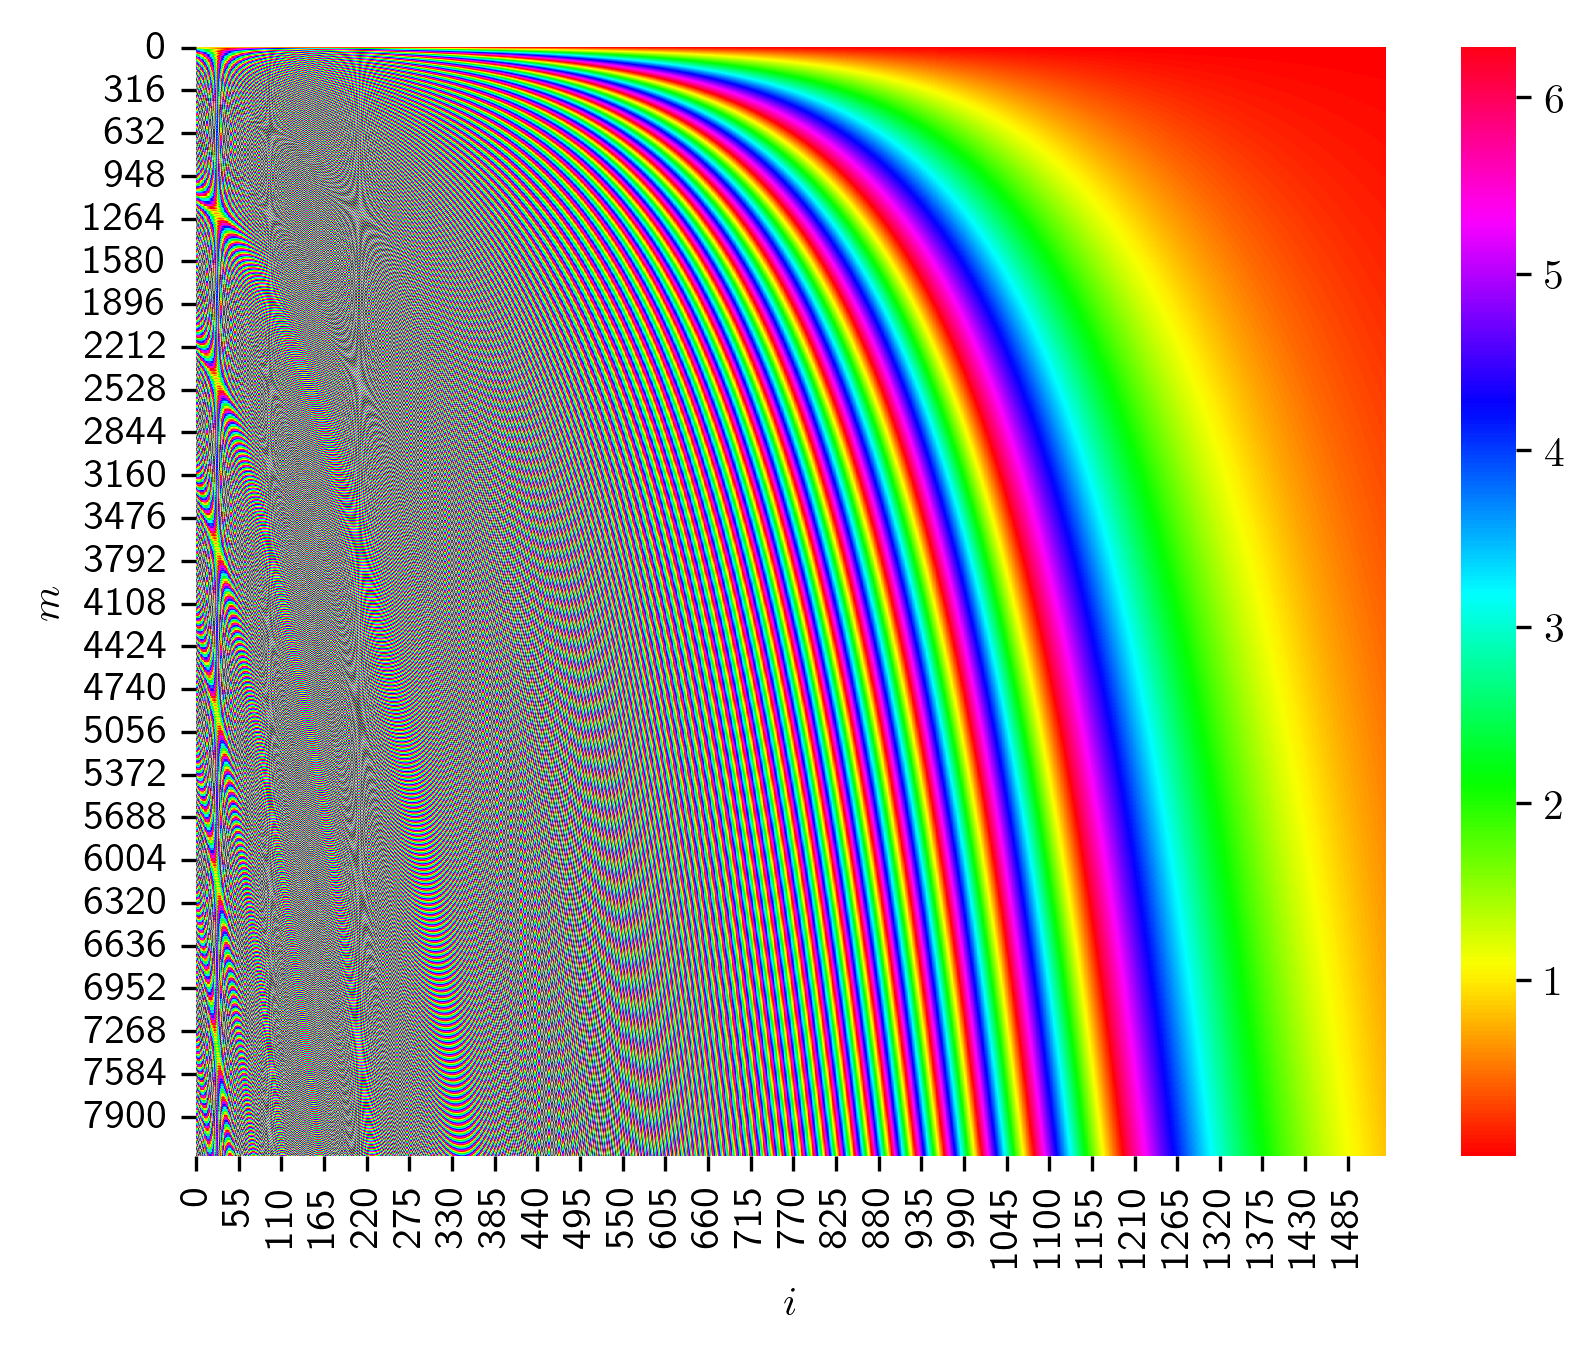
\includegraphics[width=0.8\linewidth]{rope.png}
            \caption{
                RoPEのの回転角$m\theta_i$
            }
        \end{figure}
        図を見ると、各ベクトルにおいて、
        高次元の部分には位置エンコーディングの情報が乗っていないことがわかる。
        これを踏まえると、
        次の二つの可能性を感じるため、調査を続けたい。

        \paragraph{位置エンコーディングの情報量を増やして性能が向上する場合}
            よりベクトル全体に情報を乗せる「効率的」な位置エンコーディング
        \paragraph{情報量が少ない位置エンコーディングで十分な場合}
            よりスパースな、計算量を削減できる位置エンコーディング

\begin{thebibliography}{99}
    \bibitem{attention}{
        Ashish V., et al.,
        ``Attention Is All You Need'',
        arXiv:1706.03762,
        2017
    }
    \bibitem{catastrophie}{
        Cheng-Zhi A. H., et al.,
        ``Music Transformer'',
        arXiv:1809.04281,
        2018
    }
    \bibitem{relative}{
        Peter S., et al.,
        ``Self-Attention with Relative Position Representations'',
        arXiv:1803.02155,
        2018
    }
    \bibitem{rope}{
        Jianlin S., et al.,
        ``RoFormer: Enhanced Transformer with Rotary Position Embedding'',
        arXiv:2104.09864,
        2021
    }
    \bibitem{kaiokendev}{
        kaiokendev,
        ``Extending Context is Hard... but not Impossible'',
        kaiokendev.github.io,
        ``https://kaiokendev.github.io/context'',
        最終閲覧: 2024/5/17
    }
    \bibitem{qiita}{
        masaki\_kitayama,
        ``Transformerにおける相対位置エンコーディングを理解する。'',
        Qiita,
        `https://qiita.com/masaki\_kitayama/items/01a214c07b2efa8aed1b',
        最終閲覧: 2024/5/17
    }
\end{thebibliography}
\end{document}